\subsection{The $D_{\alpha}$ array}\label{sec:dalpha_array}

Neutral particle density profiles are determined by modelling the neutral particle dynamics from particle sources and sinks which are constrained by the measurement of deuterium Balmer-alpha (or $D_{\alpha}$) emissions arising from the $n=3$ to $n=2$ transition. $D_{\alpha}$ emission occurs when a deuterium atom is excited to a higher state, usually through electron impact excitation or charge exchange. The associated radiance can be calculated as,
\begin{align}
    R &= \int_C \frac{\Delta \Omega(\vec{r})}{4\pi}\gamma_{D_{alpha}}(\vec{r}) dl\\
    \gamma_{D_{alpha}} &= \frac{A_{32}}{ A_{32} + A_{31} }\left( n_0 n_e <\sigma v>_{\text{excitation}} + n_0 n_i <\sigma v>_{\text{CX}} \right)
\end{align}
% You call this quantity "the rate of photon generation," but a check of the units shows that it has units of m^-3/s. I suspect that this is the number of photons produced per volume. The usual radiometric quantity to report here is the "radiance" which has units of Watts/(m^2 Sr). This is the amount of radiant energy emitted from a surface per solid angle per time. It may make sense to write this quantity out in terms of the line-integrated emission coefficient (units of W/(m^3 Sr)) since this is what you are measuring and forward-modelling in DEGAS2.
%--
%Changed, although what DEGAS2 does is much more complicated than this integral as it uses sub-chords and calculating percent contribution of a finite volume and so on. The complications is partly why I chose originally to present the photon generation per volume per time calculation. --Xing
where $n_0$ is the neutral density, and $<\sigma v>$ are the distribution averaged reaction rates for electron impact excitation and charge exchange into the neutral deuterium $n=3$ excited state and $A_{32}$ and $A_{31}$ are the Einstein coefficients for spontaneous emission. Given $n_e$, $n_i$, and $n_0$, the neutral emission is easy to calculate, but it varies over $3$ orders of magnitude across the plasma diameter as very little emission arising from the hot core. Accurately determining the neutral density in the core requires careful calculations of the neutral dynamics which are discussed in detail in section \ref{sec:DEGAS2}.


\begin{figure}[!htb]
	\centering
	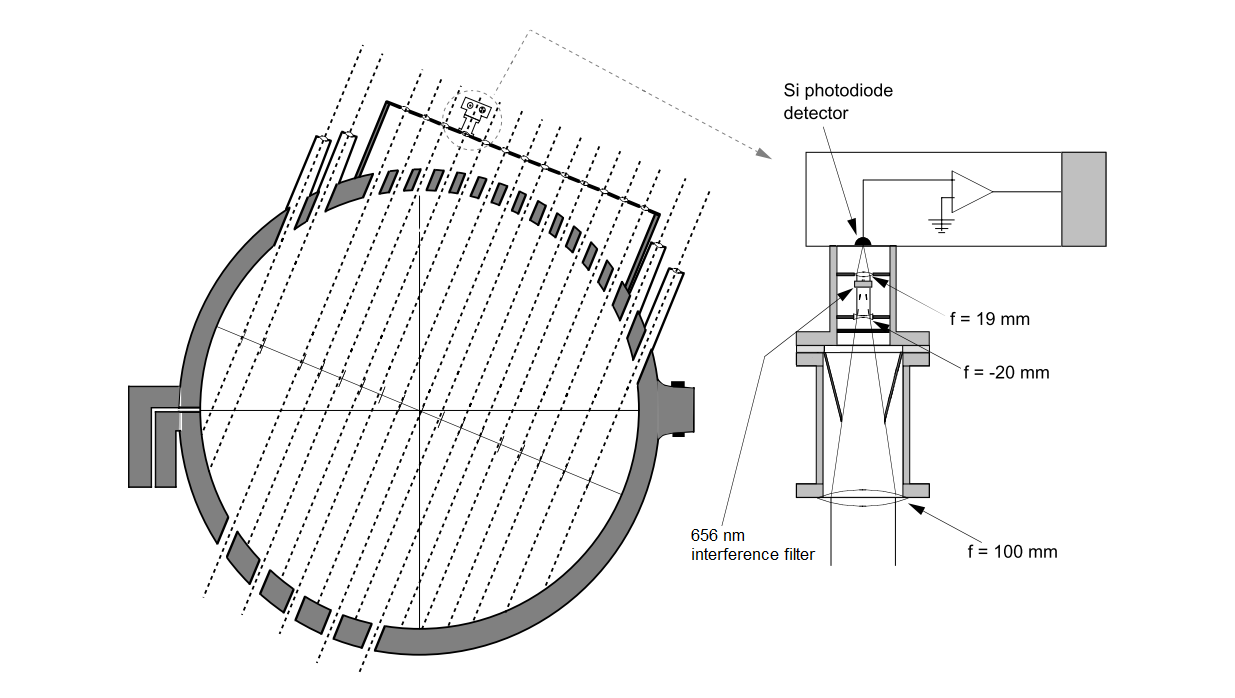
\includegraphics[width = 0.9\linewidth]{./implementation/d_alpha_detector.PNG}
	\caption[$D_{\alpha}$ detectors]{Diagram $D_{\alpha}$ detectors and available viewing chords. The detectors consist of focusing optics, a silicon photo-diode, and a trans-amplifier circuit. In some detectors there is also a pin-hole aperture used to reduce the intensity of incident light on the detector. Five of the viewing cords have matching ports on the other side, but they are not used for this work. (Reproduced with modifications from J. Anderson\cite{Anderson2001})}
	\label{fig:D_alpha_diagram}
\end{figure}

MST uses 13 silicon photo-diode detectors to observe the 656nm $D_\alpha$ line.  The detector array (referred to as the $D_{\alpha}$ array) is located at the $210 \degree$ toroidal boxport. The boxport has 17 available lines of sight, hence we are limited by the avaliable detectors. The detectors consist of filtered silicon photo diodes with a built-in current-to-voltage transimpedance amplifier. Figure \ref{fig:D_alpha_diagram} shows the physical assembly of the detectors.

\begin{figure}[!htb]
	\centering
	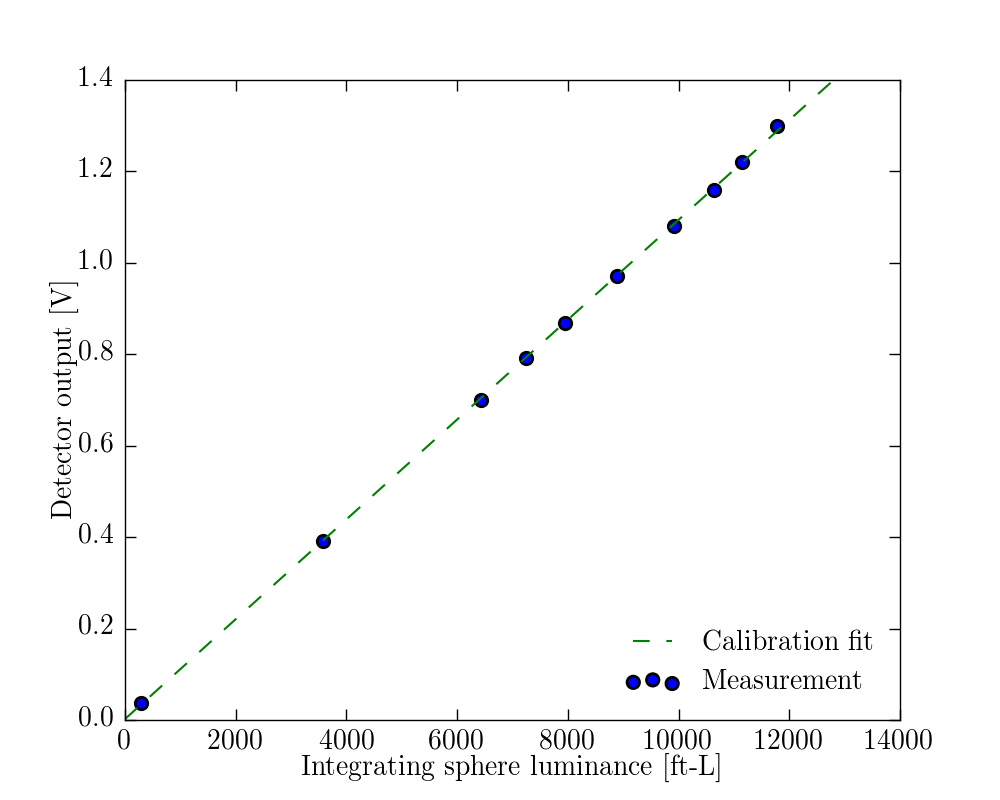
\includegraphics[width = 0.9\linewidth]{./implementation/diagnostics/l_vs_v.png}
	\caption[Example $D_{\alpha}$ calibration]{Example voltage vs luminance calibration for $D_{\alpha}$ detectors. This in particular is from detector \#32's calibration from Aug. 2015.}
	\label{fig:l_vs_v}
\end{figure}

The detectors are calibrated using a commercially available Tungsten strip-lamp with integrating sphere which has been calibrated for radiance measurements. An optical assembly identical to that on MST is used to couple light from the integrating sphere to the detector. Since the optical geometry is reproduced, the geometrical effects quantified by the {\'e}tendu $A\Delta\Omega$ are held to be constant between calibration and machine. However, the transfer function is much wider than the $H_{\alpha}$ emission line, and thus needs to be taken into account. Namely the voltage measured in calibration is
\begin{align}
    V_{\text{cal}} &= c A \Delta\Omega \int^{\infty}_{0}f(\lambda)R_\lambda(\lambda)\ d\lambda\\
    &\equiv c'R
\end{align}
where $c$ and $c'$ are calibration factors, $f(\lambda)$ is the transfer function of filter, and $R_\lambda$ is the spectral radiance of the integrating sphere. With $c'$ thus defined, it can be easily calculated from measured pairs of output voltage {\em vs} luminance slope from,
\begin{align}
    c' &= \frac{V_{\text{cal}}}{R}\\
    &= \frac{\Delta V}{\Delta L}\left(\frac{L}{R}\right)_{\lambda}
\end{align}
where $\frac{\Delta V}{\Delta L}$ is the measured voltage vs. luminance slope (see Figure \ref{fig:l_vs_v}), and $(\frac{L}{R})_{\lambda}$ is the luminance to spectral radiance conversion factor provided by NIST-certified calibration of the light source. To apply to measurements, however, we have to further consider that the voltage due to measurement of plasma emission is
\begin{align}
    V_{\text{meas}} &= c A\Delta\Omega\int^{\infty}_0\int_{C} f(\lambda)\epsilon(\lambda,l)\ dld\lambda
\end{align}
where C is the view path, l is the distance along the line-of-sight, and $\epsilon$ is the spectral emissivity. Since the plasma emission is a discrete emission line and the calibrated light source is a broad-spectrum source, we cannot equate the integration over spectral wavelength between the calibration and plasma measurements. Thus, an additional factor is needed. Approximating the spectral emissivity as a delta function, {\em i.e.} $\epsilon\approx I_{D_{\alpha}}(l)\delta(\lambda - \lambda_{D_{\alpha}})$ where $I_{D_\alpha}$ is the emissivity, the measured voltage becomes
\begin{align}
    V_{\text{meas}} &= c A\Delta\Omega f(\lambda_{D_{\alpha}}) \int_{C}I_{D_{\alpha}}(l)\ dl \nonumber\\
    &= c' \frac{f(\lambda_{D_{\alpha}})}{\int_0^{\infty}f(\lambda)d\lambda}\int_C I_{\dal}(l)\ dl \\
    &\equiv c' c_{\text{trans}}\int_C I_{\dal}(l)\ dl 
\end{align}
where in addition of the calibration factor $c'$ defined previously, the transfer function normalization factor $c_{\text{trans}} \equiv \frac{f(\lambda_{D_{\alpha}})}{\int_0^{\infty}f(\lambda)d\lambda}$ is also need for the proper calculation of the line emission intensity. This latter factor $c_{\text{trans}}$ was precisely measured using a high-resolution Ocean Optics HR2000+ spectrometer as the transfer function of the filters showed noticeable variations\cite{Eilerman}, but it is not regularly re-calibrated as it would require disassembly of the detectors. The radiance calibration of $c'$ using the integrating sphere is performed once a year during the data taking period for this work. More details of the hardware and calibration process can be found in Anderson's Ph.D. thesis\cite{Anderson2001} (Chapter 2) and Eilerman's Ph.D. thesis\cite{Eilerman} (Appendix A).